
架构和敏捷开发似乎是对立的,并且围绕着这个主题有许多神话。为了以敏捷的方式开发产品,并且还要关注架构,需要遵循一些简单的原则。

Agile, by nature, is iterative and incremental. This means preparing a big, upfront design is not an option in an Agile approach to architecture. Instead, a small, but still reasonable upfront design should be proposed. It's best if it comes with a log of decisions with the rationale for each of them. This way, if the product vision changes, the architecture can evolve with it. To support frequent release delivery, the upfront design should then be updated incrementally. Architecture developed this way is called evolutionary architecture.

Managing architecture doesn't need to mean keeping massive documentation. In fact, documentation should cover only what's essential as this way it's easier to keep it up to date. It should be simple and cover only the relevant views of the system.

There's also the myth of the architect as the single source of truth and the ultimate decisionmaker. In Agile environments, it's the teams who are making decisions. Having said that, it's crucial that the stakeholders are contributing to the decision-making process – after all, their points of view shape how the solution should look.

An architect should remain part of the development team as often they're bringing strong technical expertise and years of experience to the table. They should also take part in making estimations and plan the architecture changes needed before each iteration.

In order for your team to remain Agile, you should think of ways to work efficiently and only on what's important. A good idea to embrace to achieve those goals is domain-driven design.


\subsubsubsection{1.5.1\hspace{0.2cm}Domain-driven design}

Domain-driven design, or DDD for short, is a term introduced by Eric Evans in his book of the same title. In essence, it's about improving communication between business and engineering and bringing the developers' attention to the domain model. Basing the implementation of this model often leads to designs that are easier to understand and evolve together with the model changes.

What has DDD got to do with Agile? Let's recall a part of the Agile Manifesto:


\noindent
\hspace*{0.8cm}\textbf{Individuals and interactions} over processes and tools \\
\hspace*{0.8cm}\textbf{Working software} over comprehensive documentation \\
\hspace*{0.8cm}\textbf{Customer collaboration} over contract negotiation \\
\hspace*{0.8cm}\textbf{Responding to change} over following a plan

\noindent
\hspace*{0.8cm}— The Agile Manifesto


In order to make the proper design decisions, you must understand the domain first. To do so, you'll need to talk to people a lot and encourage your developer teams to narrow the gap between them and business people. The concepts in the code should be named after entities that are part of ubiquitous language. It's basically the common part of business experts' jargon and technical experts' jargon. Countless misunderstandings can be caused by each of these groups using terms that the other understands differently, leading to flaws in business logic implementations and often subtle bugs. Naming things with care and using terms agreed by both groups can mean bliss for the project. Having a business analyst or other business domain experts as part of the team can help a lot here.

If you're modeling a bigger system, it might be hard to make all the terms mean the same to different teams. This is because each of those teams really operates in a different context. DDD proposes the use of bounded contexts to deal with this. If you're modeling, say, an ecommerce system, you might want to think of the terms just in terms of a shopping context, but upon a closer look, you may discover that the inventory, delivery, and accounting teams actually all have their own models and terms.

Each of those is a different subdomain of your e-commerce domain. Ideally, each can be mapped to its own bounded context – a part of your system with its own vocabulary. It's important to set clear boundaries of such contexts when splitting your solution into smaller modules. Just like its context, each module has clear responsibilities, its own database schema, and its own code base. To help communicate between the teams in larger systems, you might want to introduce a context map, which will show how the terms from different contexts relate to each other:

\begin{center}
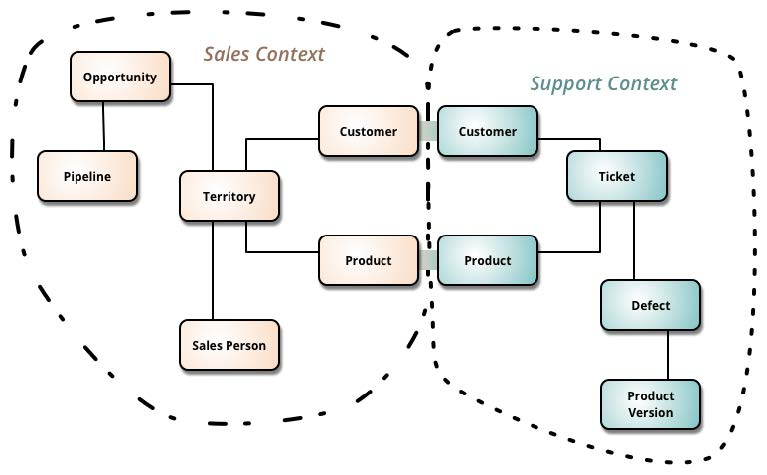
\includegraphics[width=0.9\textwidth]{content/1/chapter1/images/1.jpg}\\
Figure 1.1 – Two bounding contexts with the matching terms mapped between them (image from one of Martin Fowler's articles on DDD: \url{https://martinfowler.com/bliki/BoundedContext.html})
\end{center}

As you now understand some of the important project-management topics, we can switch to a few more technical ones.








